\documentclass[../../main]{subfiles}
\graphicspath{{\subfix{../../Images/}}}

\begin{document}

W tej części pracy zostanie przedstawiona dekompozycja oprogramowania systemowego omówionego w poprzedniej części w architekturach z systemem operacyjnym i wirtualizacją, a konkretnie: systemu operacyjnego i hiperwizora. Następnie oprogramowanie odpowiadające za zarządzanie dostępem do zasobów jednostki obliczeniowej zostanie wyodrębnione ze wspomnianego wcześniej oprogramowania systemowego dla przeprowadzenia analizy w następnej części pracy.

Należy zauważyć, że celem tej pracy nie jest omówienie wszystkich elementów oprogramowania systemowego. Pozostałe elementy oprogramowania systemowego będą wspomniane, jeżeli zajdzie potrzeba, tylko w sposób ogólny, w celu prześledzenie udziału oprogramowania zarządzającego zasobami jednostką obliczeniową w ogólnej architekturze oprogramowania systemowego, oraz umożliwienia wyodrębnienia tej części do dalszej analizy. % TODO: check first centense punktuation and structure.

\subsection{Dekompozycja}

Jak wspomniano wcześniej, z punktu widzenia zarządzania zasobami jednostki obliczeniowej szczególnie interesujące są dwa rodzaje oprogramowania systemowego: system operacyjny i hiperwizor. Na \cref{fig:cpu-resources-mult} przedstawiono przydzielenie zasobów jednostki obliczeniowej za pomocą tego oprogramowania systemowego. Kolorami zaznaczone są tryby, w których znajduje się jednostka obliczeniowa podczas wykonywania instrukcji przez określone oprogramowanie, a zacieniony obszar wskazuje, że serwisy systemu operacyjnego mogą być wykonywane zarówno w trybie jądra, jak i w trybie aplikacji. Strzałkami zaznaczono przydzielenie zasobów jednostki obliczeniowej do określonego oprogramowania przez odpowiednią logikę w oprogramowaniu systemowym.

\begin{figure}[ht]
    \centering
    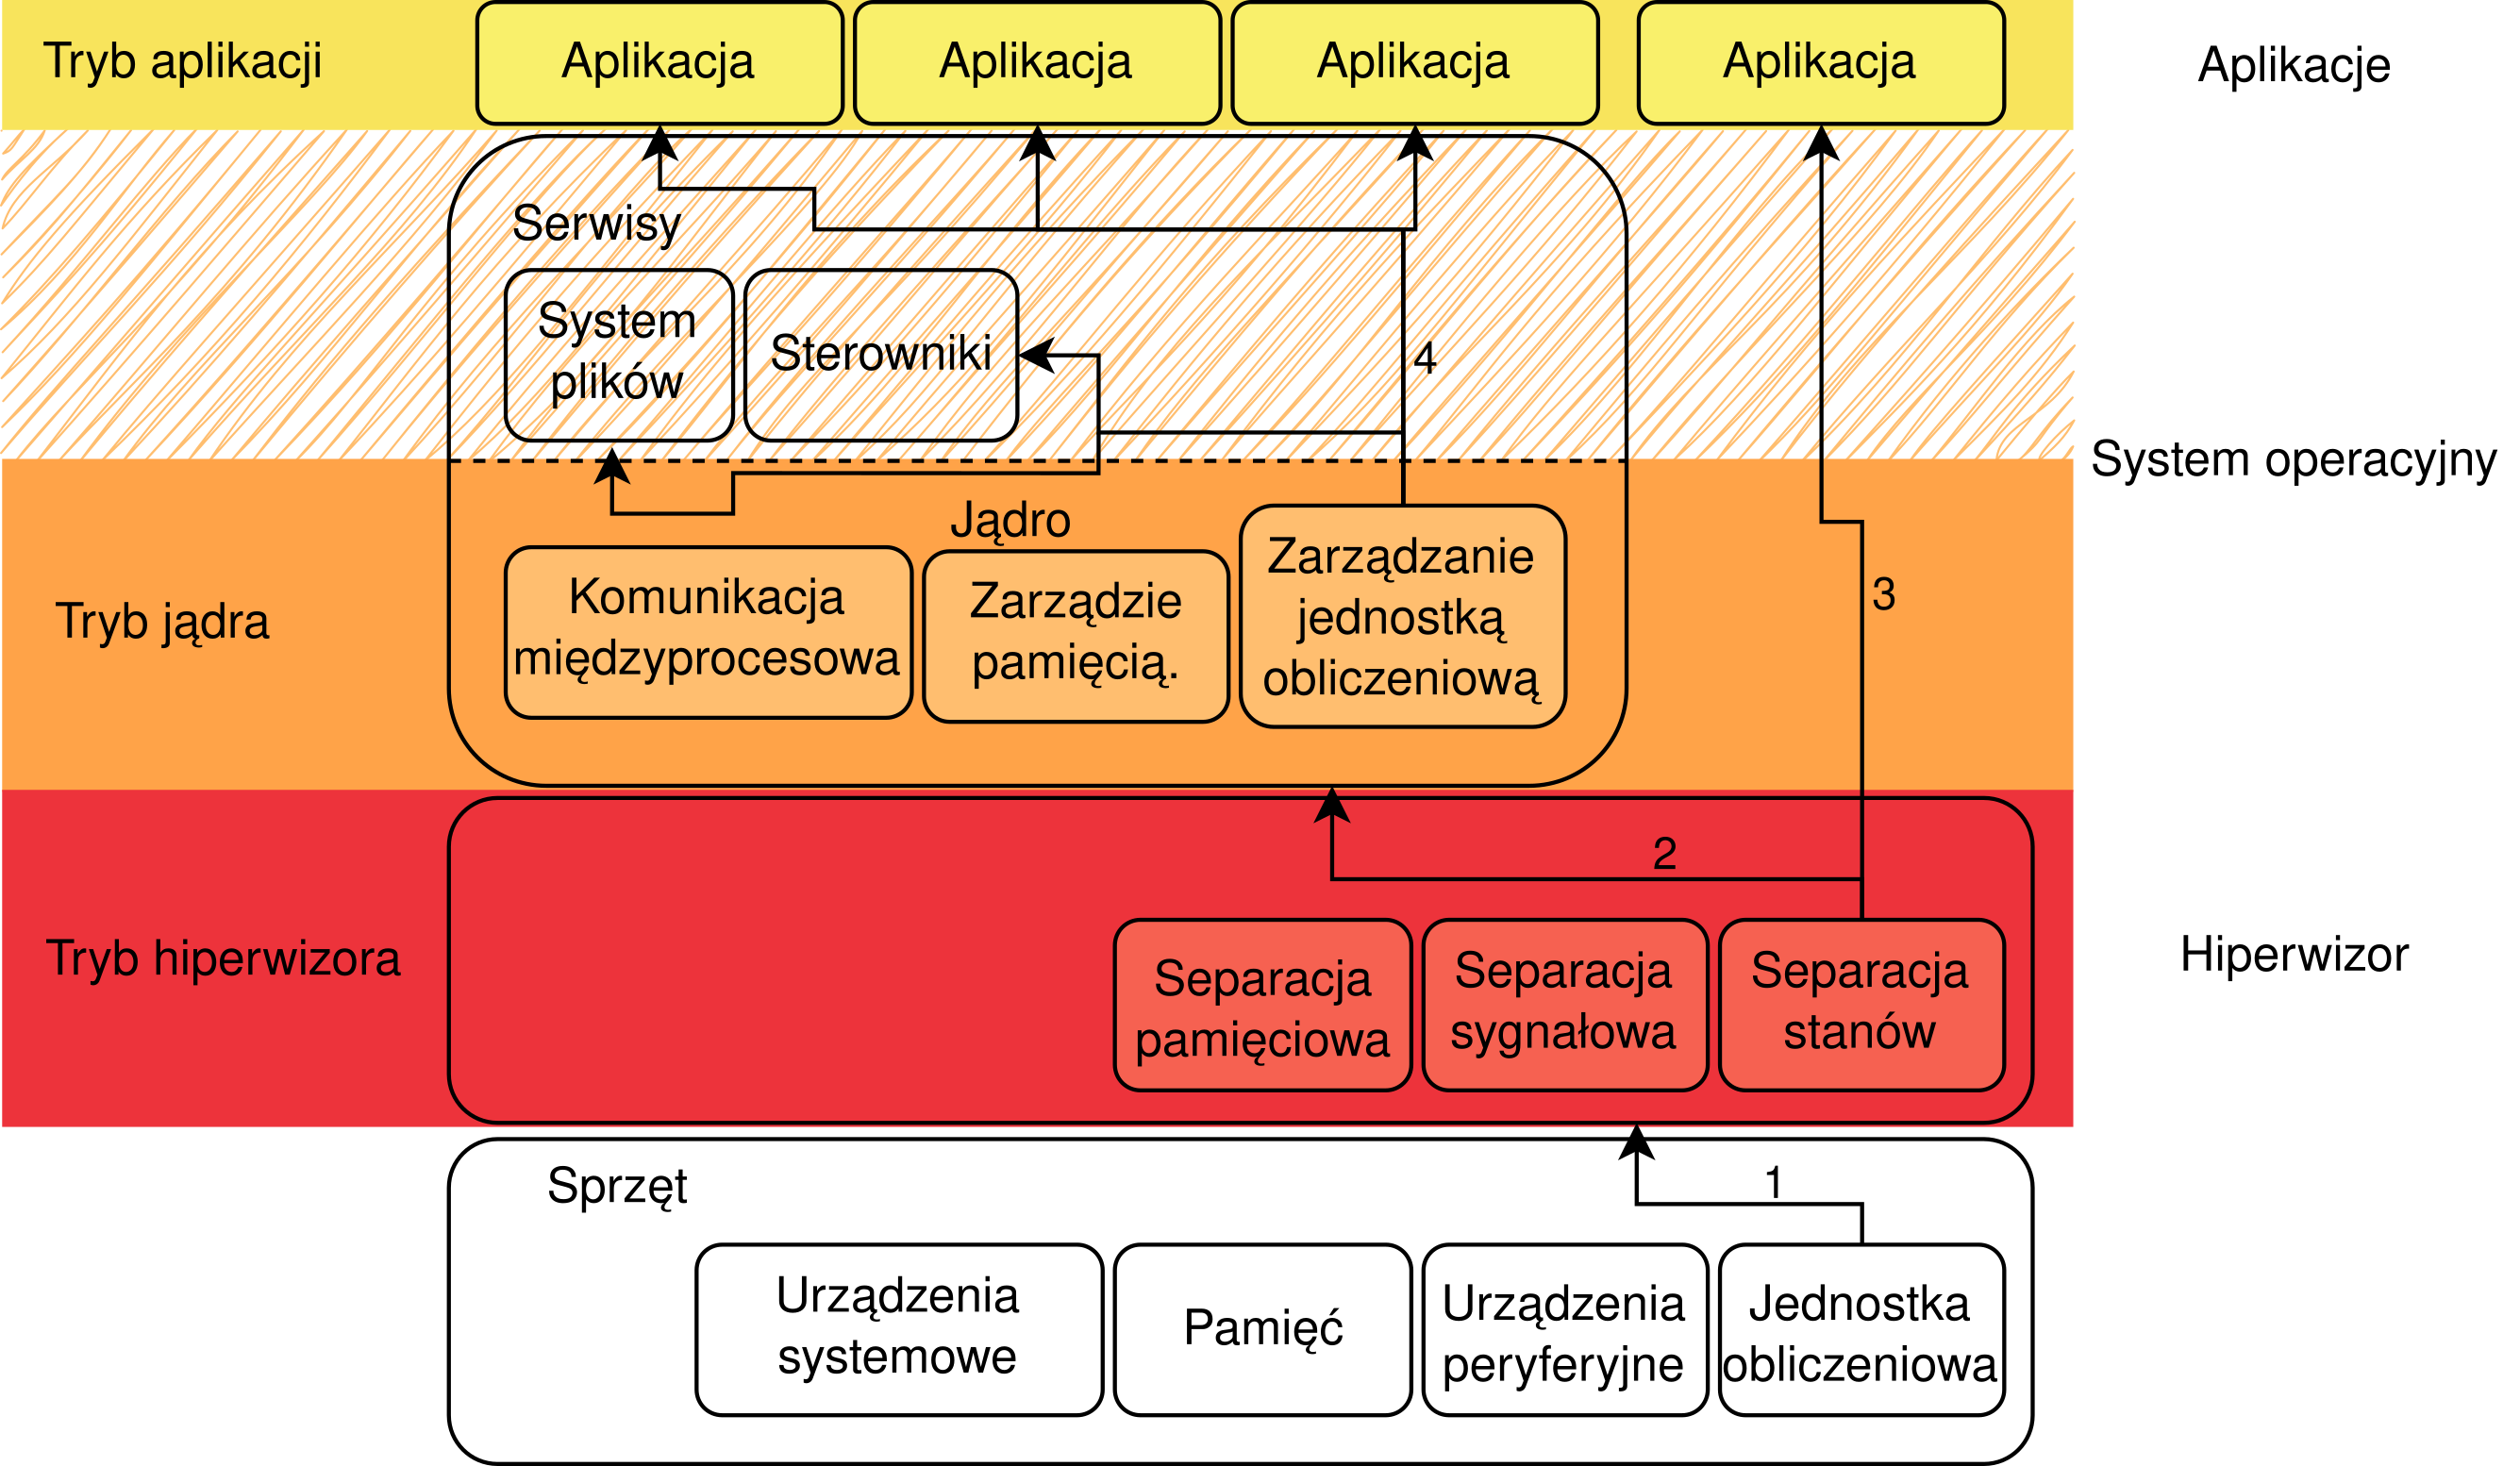
\includegraphics[width=\textwidth]{Images/cpu-resources-multiplexing.png}
    \caption{Przydzielenie dostępu do zasobów jednostki obliczeniowej przez oprogramowanie systemowe: system operacyjny i hiperwizor}
    \label{fig:cpu-resources-mult}
\end{figure}

Ten rysunek ilustruje architekturę z wirtualizacją, podczas gdy architektura bez wirtualizacji wykorzystująca jedynie system operacyjny, może być przedstawiona usuwając z \cref{fig:cpu-resources-mult} cały hiperwizor i strzałkę o numerze 3. W takim przypadku strzałka o numerze 1 będzie wskazywać bezpośrednio na jądro systemu operacyjnego.

Jest to struktura hierarchiczna, tzn. (numery punktów są odpowiednie do numerów strzałek na \cref{fig:cpu-resources-mult}):

\begin{enumerate}
    \item Hiperwizor otrzymuje kontrolę nad wszystkimi zasobami jednostki obliczeniowej i przydziela je do oprogramowania, które on uruchamia: system operacyjny (strzałka nr 2 na \cref{fig:cpu-resources-mult}) lub aplikacja (strzałka nr 3 na \cref{fig:cpu-resources-mult}).
    \item System operacyjny otrzymuję od hiperwizora pewną część zasobów jednostki obliczeniowej (strzałka nr 2 na \cref{fig:cpu-resources-mult}) i przydziela je do serwisów lub aplikacji (strzałki o wspólnym numerze 4 na \cref{fig:cpu-resources-mult}).
    \item Aplikacja uruchomiona bez systemu operacyjnego otrzymuje przydzielone zasoby od hiperwizora (strzałka nr 3 na \cref{fig:cpu-resources-mult}) i zaczyna wykonywać swoją pracę.
    \item Aplikację i serwisy uruchomione przez system operacyjny, otrzymują przydzielone im zasoby przez system operacyjny (strzałki o wspólnym numerze 4 na \cref{fig:cpu-resources-mult}) i zaczynają wykonywać swoją pracę.
\end{enumerate}

W systemie operacyjnym funkcjonalność przydzielenia zasobów jednostki obliczeniowej jest jedną z trzech kluczowych, pozostałe dwie to: komunikacja międzyprocesowa i zarządzanie pamięcią. Natomiast w hiperwizorze jest to jeden ze sposobów separacji, pozostałe dwa to: separacja sygnałowa i separacja pamięciowa. Wytłumaczenie separacji jest zamieszczone w \hyperref[sec:zalacznik-2]{załączniku nr 2}).

Logikę lub kod, który odpowiada za zarządzanie zasobami jednostki obliczeniowej zarówno w systemie operacyjnym, jak i hiperwizorze (pomiędzy strzałkami 1 i 2, oraz pomiędzy strzałkami 2 i 4, \cref{fig:armv8-m-context-switch}) można nazwać nadzorcą (ang. supervisor). Takie nazewnictwo będzie stosowane w dalszej części pracy. Nadzorcę można także podzielić na dwie części: dyspozytora (ang. dispatcher) i planistę (ang. scheduler). Centrum uwagi tej pracy jest planista.
\newpage

\subsection{Wyodrębnienie}

Wspomniany w poprzedniej części nadzorca jest wywoływany tylko w pewnych, szczególnie zdefiniowanych przypadkach, aby wykonać przełączenie kontekstu. Wywoływany on może być periodycznie, za pomocą periodycznego przerwania, lub "na żądanie" za pomocą przerwania systemowego. W przypadku \gls{arm}'u są to przerwania generowane instrukcjami \gls{svc} i \gls{hvc}.

\begin{figure}[H]
    \centering
    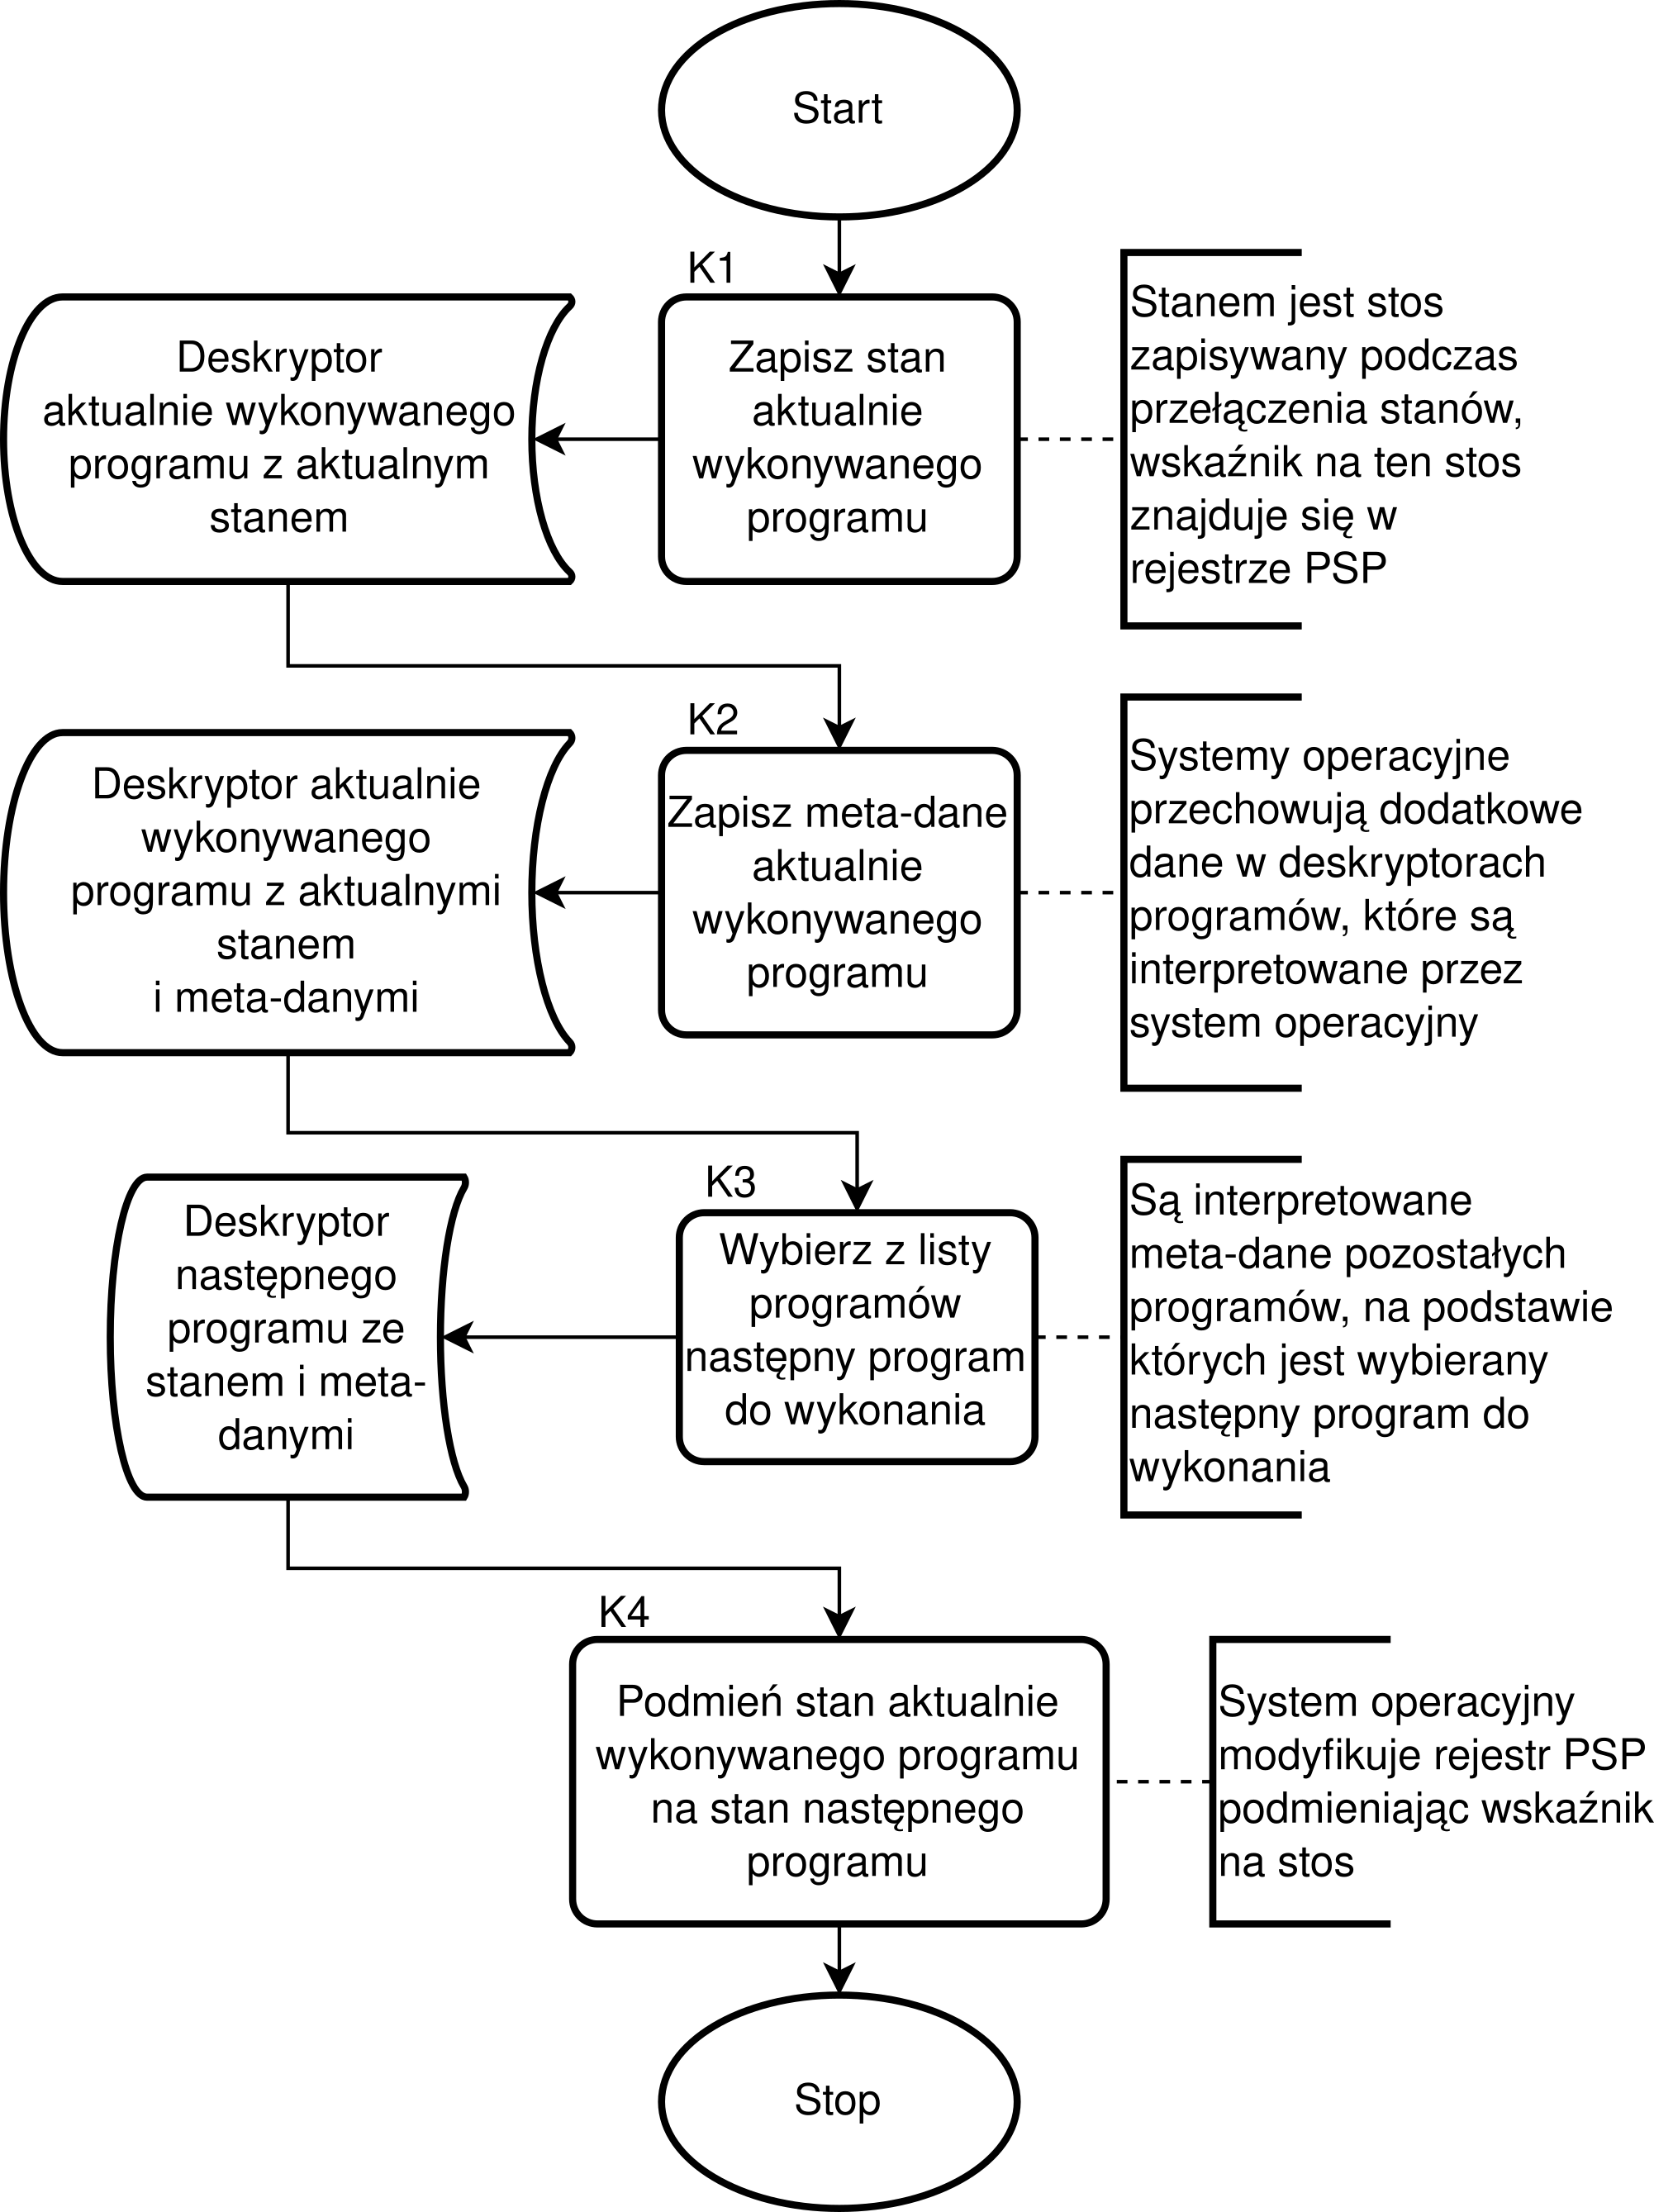
\includegraphics[width=0.85\textwidth]{Images/context-switching-armv8-m.png}
    \caption{Ogólna logika przełączenia kontekstu}
    \label{fig:armv8-m-context-switch}
\end{figure}

Po wywołaniu nadzorcy następuje przełączenie kontekstu. Na \cref{fig:armv8-m-context-switch} ogólnie opisane są kroki przełączania kontekstu. Przy czym kroki \textit{K1}, \textit{K2} i \textit{K4} (\cref{fig:armv8-m-context-switch}) są wykonywane przez dyspozytora, a tylko krok \textit{K3} (\cref{fig:armv8-m-context-switch}) jest wykonywany przez planistę.

Zadaniem dyspozytora jest otrzymywanie informacji i przekierowanie jej w odpowiednim formacie do planisty (kroki \textit{K1} i \textit{K2} na \cref{fig:armv8-m-context-switch}), który podejmuje decyzję na podstawie zdefiniowanych reguł (krok \textit{K3} na \cref{fig:armv8-m-context-switch}), i informuje o tym dyspozytora. Dyspozytor podejmuje odpowiednie dla podjętej decyzji działania (krok \textit{K4} na \cref{fig:armv8-m-context-switch}).

Wejściem do planisty jest lista deskryptorów procesów oczekujących na przydzielenie zasobów obliczeniowych oraz ilość dostępnych zasobów obliczeniowych. Wyjściem jest deskryptor procesu z przydzielonymi zasobami jednostki obliczeniowej. Planista podejmuje decyzję na podstawie wstępnie zdefiniowanych reguł. Reguły te będą omówione w następnej części pracy.

\end{document}